\graphicspath{{figs/3a}}
\chapter{Bayesian Linear Regression}

In this chapter, we delve into Bayesian Linear Regression, a fundamental concept in Bayesian Deep Learning. After discussing the general landscape of deep learning technologies and acknowledging the associated challenges, including problems related to interpretability and uncertainty in predictions, we turn our attention to Bayesian models. Bayesian Linear Regression serves as an ideal starting point for understanding Bayesian methods due to its relative simplicity and the availability of a closed-form solution for its posterior distribution. The variance present in these distributions captures epistemic uncertainty, setting it apart from the deterministic single-point predictions provided by traditional neural networks. Throughout this chapter, we not only introduce the concept of Bayesian Linear Regression but also contextualize its importance within the broader framework of Bayesian Deep Learning, providing a solid foundation for comprehending Bayesian approaches in machine learning.

\section{Linear Basis function model}

In this section, we introduce the fundamental concepts of Bayesian Linear Regression. We focus on laying a strong theoretical foundation, explaining the underlying mathematics, and outlining why a Bayesian approach is chosen for linear regression tasks.

\subsection{Gaussian basis functions}
\paragraph*{1.2. Recall closed form of the posterior distribution in linear case. Then, code and visualize posterior sampling. What can you observe?}

Let $N$ denote the number of training examples, $K$ the number of dimensions of the outputs, and $p$ the number of features (or predictors) in the input data. Consider $X \in \mathbb{R}^{N \times p}$, the input matrix, and $Y \in \mathbb{R}^{N \times K}$, the output matrix. 

We typically define the posterior distribution as $ p(w | X, Y) $. This distribution represents our updated beliefs about the parameters $ w $ after observing the data $ X $ and $ Y $. According to Bayes' rule, we can express the posterior distribution as the product of two components:
\begin{enumerate}
    \item $ p(w) $, which represents our prior beliefs about the distribution of $ w $ before observing the data.
    \item $ p(Y | X, w) $, indicating the probability of observing the data $ Y $ given the parameters $ w $ and the data $ X $. This quantifies how likely our data is under different hypotheses represented by $ w $.
\end{enumerate}
Therefore, the formula for the posterior distribution is given by:
\[ p(w | X, Y) \propto p(Y | X, w) p(w) \]

In this formula, we start with our initial beliefs (priors) and then update these beliefs based on the new data (likelihood). In the case of our linear model, we know that $ y_i = \Phi^T_i w + \epsilon $, with $ \Phi \in \mathbb{R}^{N \times (p + 1)} $ representing the design matrix and $ \epsilon $ denoting the residual. Assuming that the error follows a centered Gaussian distribution with standard deviation $ \beta ^{-1} = 2\sigma^2 $, meaning that $ \epsilon \sim \mathcal{N}(0, \beta ^{-1}) $. Consequently, we can conclude that:
\[ p(y_i | x_i, w) \sim \mathcal{N}(\Phi^T_i w, \beta ^{-1}) \]

Furthermore, we selected a centered Gaussian prior with a variance of $ \alpha^{-1}I $ where $\alpha$ governs the prior distribution over the weights $\mathbf{w}$:
\[ p(w | \alpha) \sim \mathcal{N}(0, \alpha^{-1}I) \]

In this specific case, we can demonstrate that the posterior distribution $ p(w | X, Y) $ follows a Gaussian distribution as follows:
\[ p(w | X, Y) \sim \mathcal{N}(\boldsymbol{\mu}, \boldsymbol{\Sigma}) \]

The precision matrix $ \boldsymbol{\Sigma} $, which is the inverse of the covariance matrix of the distribution parameters, is defined as:
\[ \boldsymbol{\Sigma}^{-1} = \alpha I + \beta \Phi^T \Phi \]

\noindent The mean of the distribution parameters is given by:
\[ \boldsymbol{\mu} = \beta \boldsymbol{\Sigma} \Phi^T Y \]

Parameters $\alpha$ and $\beta$ serve analogous roles, with $\alpha$ governing the prior distribution and $\beta$ regulating the likelihood.

Now, we can proceed to sample from the updated (with data) posterior distribution $p(w | X, Y)$. This process is demonstrated in \Cref{fig:posterior}, with $\alpha = 2$ and $\beta = (2 \times 0.2^2)^{-1}$. It is worth noting that when $N=0$, the posterior distribution $p(w|X,Y)$ simplifies to the prior distribution $p(w)$. As we increase the number of data points, we can observe how the model's certainty increase, demonstrated by the reduction in the variance of the parameters of the distribution. In other words, having more data points reduces aleatoric uncertainty.

\begin{figure}[H]
    \centering
    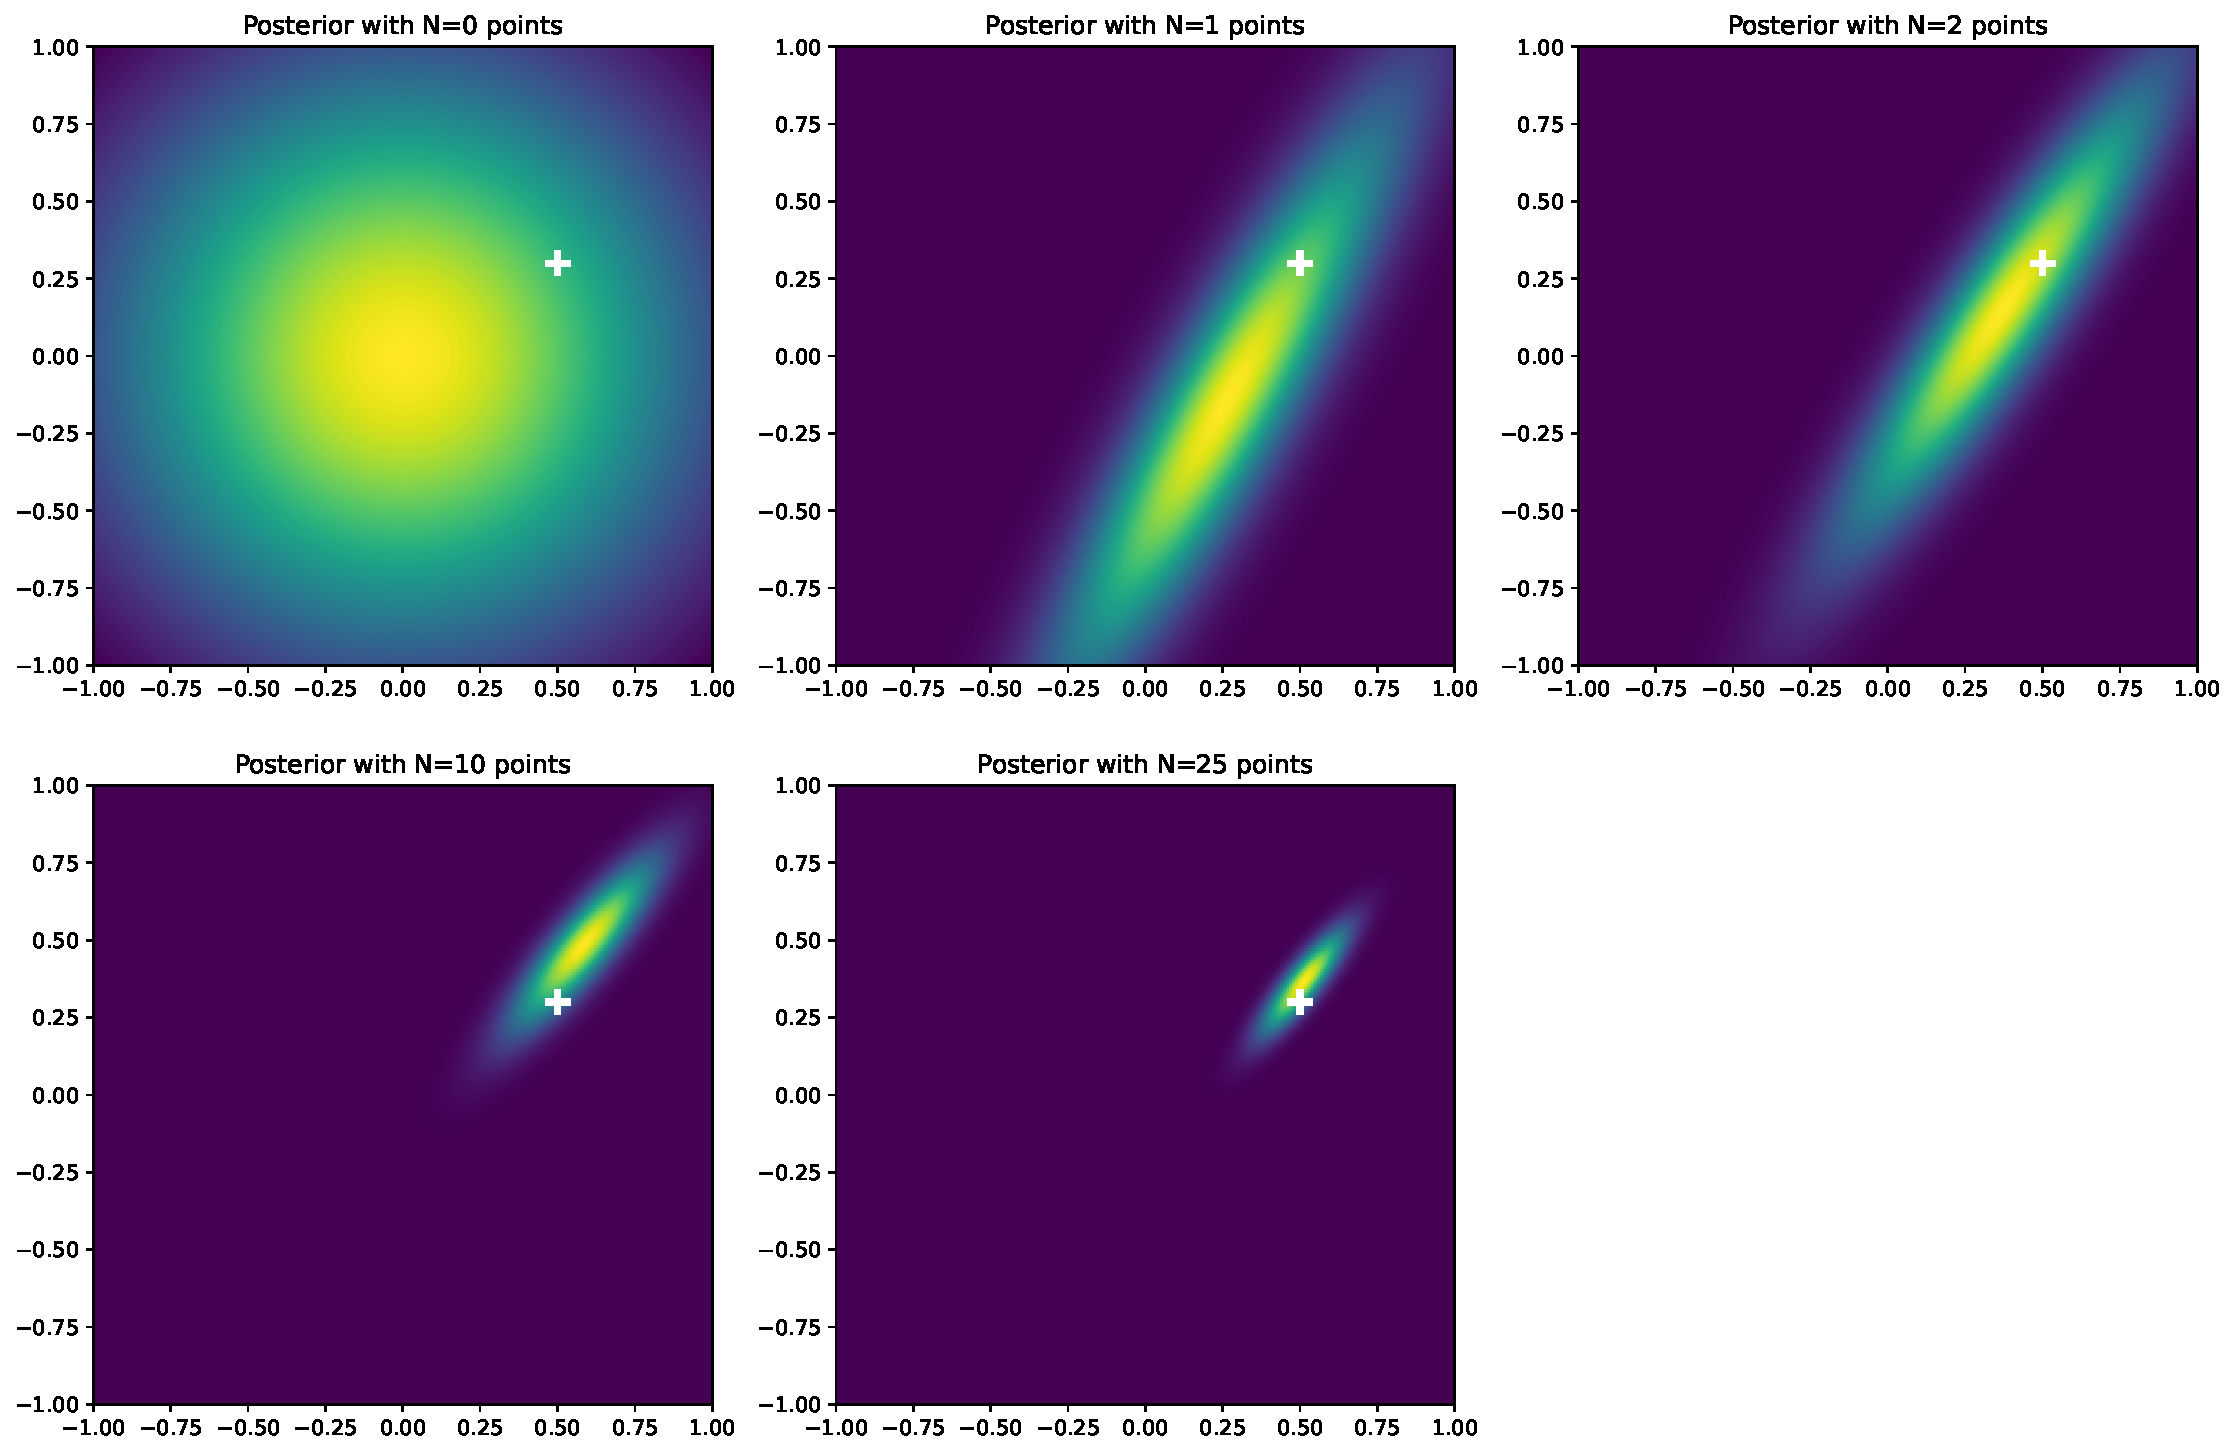
\includegraphics[width=0.95\textwidth]{posterior.pdf}
    \caption{Evolution of a Bayesian posterior distribution with increasing data points: A visual representation of Bayesian inference, depicting how the posterior distribution updates as more data is incorporated. From left to right, the figures show the posterior with $N=0$ (prior distribution), $N=1$, $N=2$, $N=10$, and $N=25$ data points, respectively. The cross mark represents the ground truth.}
    \label{fig:posterior}
\end{figure}

\paragraph*{1.3. Recall and code closed form of the predictive distribution in linear case.}
Using the information from the previous question, we can now calculate the predictive distribution for new data point $x^\star$ by marginalizing over the parameter $w$. This is represented by the following equation where $\mathcal{D} = \{X,Y\}$ denotes the dataset:
\[ p(y|x^\star , \mathcal{D}, \alpha, \beta ) = \int p(y| x^\star, w, \beta)p(w| \mathcal{D}, \alpha, \beta ) \]

By leveraging the property that the convolution of two Gaussian distributions results in another Gaussian distribution, we can demonstrate that the closed-form expression for the predictive distribution in the linear case is as follows:
\[ p\left(y|x^\star; \mathcal{D}, \alpha, \beta\right) = \mathcal{N}\left(y; \mu^T \boldsymbol{\Phi}(x^\star), \frac{1}{\beta} + \boldsymbol{\Phi}(x^\star)^T \boldsymbol{\Sigma} \boldsymbol{\Phi}(x^\star)\right) \]

We can see that the variance in the predictive distribution $ \sigma ^2_{pred} $  for a new observation can be divided into two parts:
\begin{enumerate}
    \item The aleatoric uncertainty, which represents the inherent noise in the data, that we fixed around $ \beta ^{-1}$;
    \item The epistemic uncertainty related to the model parameters $ w $, characterized by $\boldsymbol{\Phi}(x^\star)^T \boldsymbol{\Sigma} \boldsymbol{\Phi}(x^\star).$
\end{enumerate}
It's worth noting that as the number of data points $N$ approaches infinity ($ \lim_{N \to \infty} \boldsymbol{\Phi}(x^\star)^T \boldsymbol{\Sigma} \boldsymbol{\Phi}(x^\star) = 0 $), our understanding of the model parameters becomes nearly perfect. In this scenario, the only remaining source of uncertainty is the aleatoric uncertainty, stemming from the noise in the data.

\paragraph*{1.4. Based on previously defined \texttt{f\_pred()}, predict on the test dataset. Then visualize results using \texttt{plot\_results()} defined at the beginning of the notebook.}
\Cref{fig:phi_linear} illustrates a comparison between the predictions made by a Bayesian Linear Regression model and the actual ground truth. In the left panel, you can see the model's linear fit to the training data, shown as blue points, alongside the true ground truth represented by the green line. To visualize the model's predictive uncertainty, shaded areas are used, ranging from dark to light, which correspond to one, two, and three standard deviation intervals, respectively.

The right panel of the figure focuses on the predictive variance $ \sigma^2_{\text{pred}}  $ along the x-axis. This variance is depicted by a curve that widens as it moves away from the center of the training data, marked by the vertical dashed line. These visual elements together provide a comprehensive view of the model's confidence in its predictions across the entire domain.
\begin{figure}[H]
    \centering
    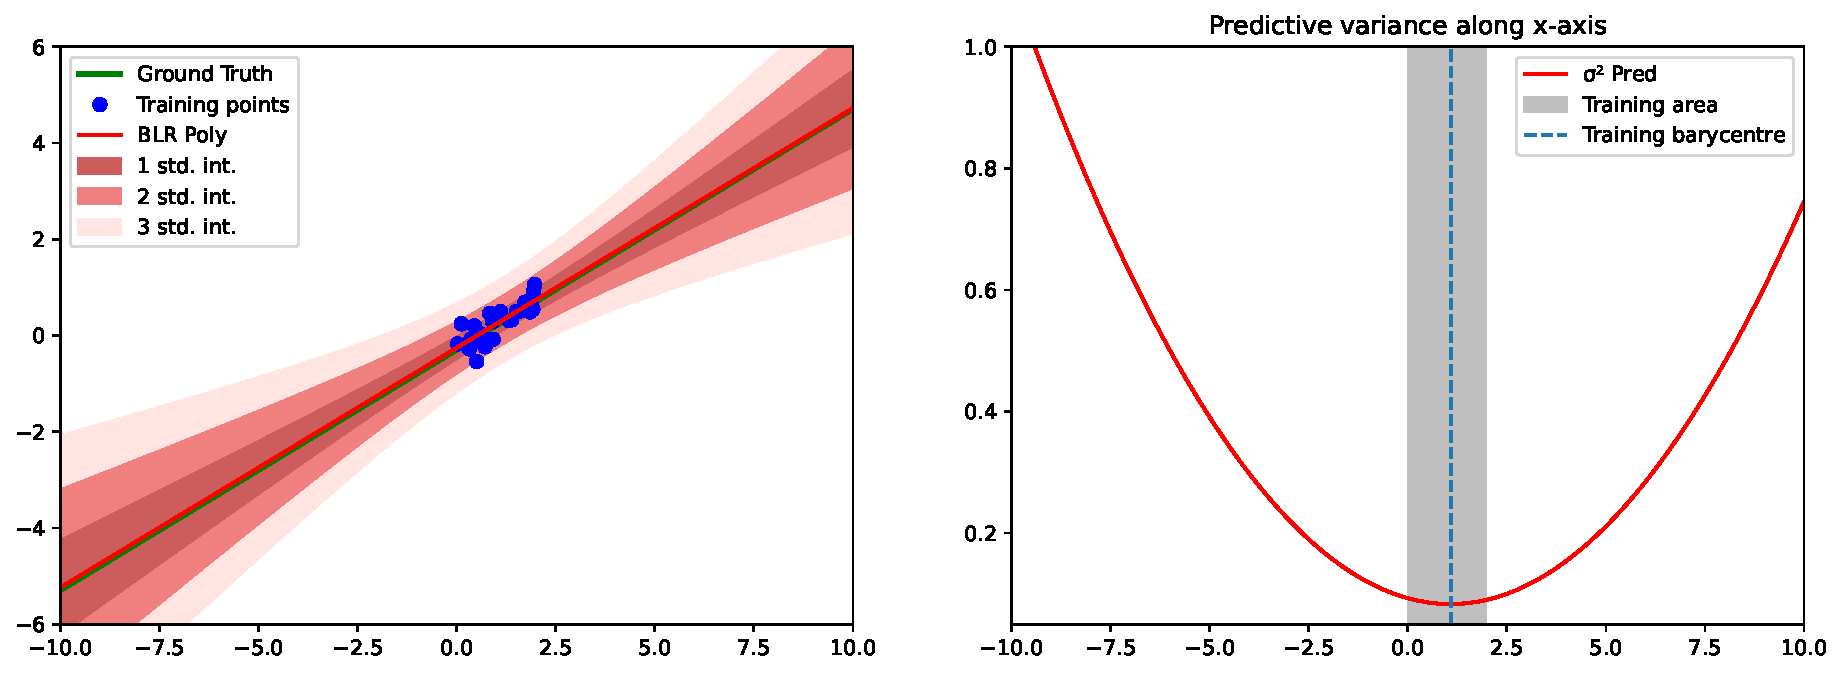
\includegraphics[width=0.95\textwidth]{phi_linear.pdf}
    \caption{Visualization of predictive distribution of a linear dataset using Bayesian Linear Regression. The left panel illustrates the fit (red line) to the training data (blue points) against the ground truth (green line). The shaded areas represent the predictive uncertainty, with one, two, and three standard deviation intervals shown in progressively lighter shades. The right panel displays the predictive variance $\sigma^2_{\text{pred}} $ across the x-axis. The vertical dashed line indicates the center of the training data.}
    \label{fig:phi_linear}
\end{figure}

\paragraph*{1.5. Analyse these results. Why predictive variance increases far from training distribution? Prove it analytically in the case where $\alpha=0$ and $\beta=1$.}

In the left panel of \Cref{fig:phi_linear}, we can observe that the confidence intervals are narrowest near the cluster of training points. This suggests higher confidence in predictions within this area. As we move away from the center of the training data (towards the extremities of the x-axis), the confidence intervals become wider, indicating increasing uncertainty in the model's predictions.

Looking at the right panel of \Cref{fig:phi_linear}, we notice that the variance remains low in the region where the training data is located (the grey shaded area). This correlates with the tight confidence intervals shown in the left panel. As expected, the predictive variance is lowest near the training barycentre, reflecting greater model certainty (i.e. lower epistemic uncertainty) in this region due to the presence of more training data points. As we move away from the training area on either side, the predictive variance increases significantly, which is consistent with the expanding confidence intervals in the left panel. This sharp increase in variance indicates a significant decrease in the model's confidence (i.e. a significant increase in the model's epistemic uncertainty) in its predictions outside the range of the training data. This pattern is expected, as the model has less points to rely on for predictions in these regions. % This is an expected pattern, as the model has less data to rely on for predictions in these regions, and we thus can not be sure about them. % Thus, the Bayesian Linear Regression model offers more reliable predictions within the training data range, with confidence diminishing as predictions move away from this range.
\vspace{\baselineskip}\linebreak
\noindent Let's prove it analytically. With $\alpha = 0$ and $\beta = 1$, the computation of $\boldsymbol{\Sigma}^{-1}$ simplifies as follows:
\begin{align*}
    \boldsymbol{\Sigma}^{-1} 
        &= 0 \cdot I_3 + 1 \cdot \Phi^T \Phi \\
        &= \Phi^T \Phi \\ 
        &= \begin{pmatrix}
            1 & \dots & 1 \\
            x_1 & \dots & x_N
        \end{pmatrix} 
        \begin{pmatrix}
            1 & x_1 \\
            \vdots & \vdots \\
            1 & x_N 
        \end{pmatrix} \\
        &= \begin{pmatrix}
            N &  \sum x_i \\
             \sum x_i &  \sum x_i^2
        \end{pmatrix}
\end{align*}
To invert $\boldsymbol{\Sigma}$, we use the classic formula for a $2 \times 2$ matrix:
\[
    \boldsymbol{\Sigma} = \frac{1}{\det \boldsymbol{\Sigma}^{-1}} \begin{pmatrix}
         \sum x_i^2 & -  \sum x_i \\
        -  \sum x_i & N
    \end{pmatrix}
\]
Returning to our expression for $ \sigma^2_{\text{pred}} = \Phi (x^\star ) ^T \boldsymbol{\Sigma} \Phi (x^\star )$, we have:
\begin{align*}
    \sigma^2_{\text{pred}} = \Phi (x^\star ) ^T \boldsymbol{\Sigma} \Phi (x^\star ) &= \frac{1}{\det \boldsymbol{\Sigma}^{-1}} \begin{pmatrix}
        1 \\
        x^\star 
    \end{pmatrix} \begin{pmatrix}
         \sum x_i^2 & -  \sum x_i \\
        -  \sum x_i & N
    \end{pmatrix}\begin{pmatrix}
        1 & x^\star 
    \end{pmatrix} \\
    &= \frac{1}{\det \boldsymbol{\Sigma}^{-1}} \begin{pmatrix} \sum x_i^2 - x^\star  \sum x_i \\ x^\star N -  \sum x_i\end{pmatrix} \begin{pmatrix}1 & x^\star \end{pmatrix} \\
    &= \frac{1}{\det \boldsymbol{\Sigma}^{-1}}\left( \sum_{i=1}^{N} x_i^2 - x^\star  \sum_{i=1}^{N} x_i + {x^\star }^2 N - x^\star  \sum_{i=1}^{N} x_i\right) \\
    &= \frac{1}{\det \boldsymbol{\Sigma}^{-1}}\left( \sum_{i=1}^{N} x_i^2 - 2 x^\star  \sum_{i=1}^{N} x_i + {x^\star }^2 N\right) \\
    &= \frac{1}{\det \boldsymbol{\Sigma}^{-1}} \sum_{i=1}^{N} \left(x_i - x^\star \right)^2
\end{align*}

This formula reveals that the predictive variance is directly proportional to epistemic uncertainty, which, in the case of our linear regression, is the squared differences between each training data point $x_i$ and the prediction point $x^\star$. As $x^\star$ moves away from the region where the training data is concentrated, these squared differences grow, consequently leading to an increase in the predictive variance.

\paragraph*{Bonus: What happens when applying Bayesian Linear Regression on the following dataset?}

Examining the right panel in \Cref{fig:phi_linear_hole}, an intriguing observation is made: the variance is unexpectedly minimized at the barycenter, i.e. the "hole" where there are no training data points. Normally, one would anticipate an increase in variance in data-scarce regions. However, this phenomenon can be explained by the fact that a point within this region is positioned closely between two clusters of training points. This proximity results in lower squared differences (epistemic uncertainty) and, as previously discussed, leads to a lower predictive variance. Additionally, due to the broader distribution of our training dataset, we observe lower predictive variance at the endpoints when compared to our previous results. This overconfidence can be attributed to our strong prior belief in the linearity of the data. In fact, we can perceive it in this way: when we draw a line between two points, we have more certainty about its direction when it passes through two distant points than through two close points.

\begin{figure}[H]
    \centering
    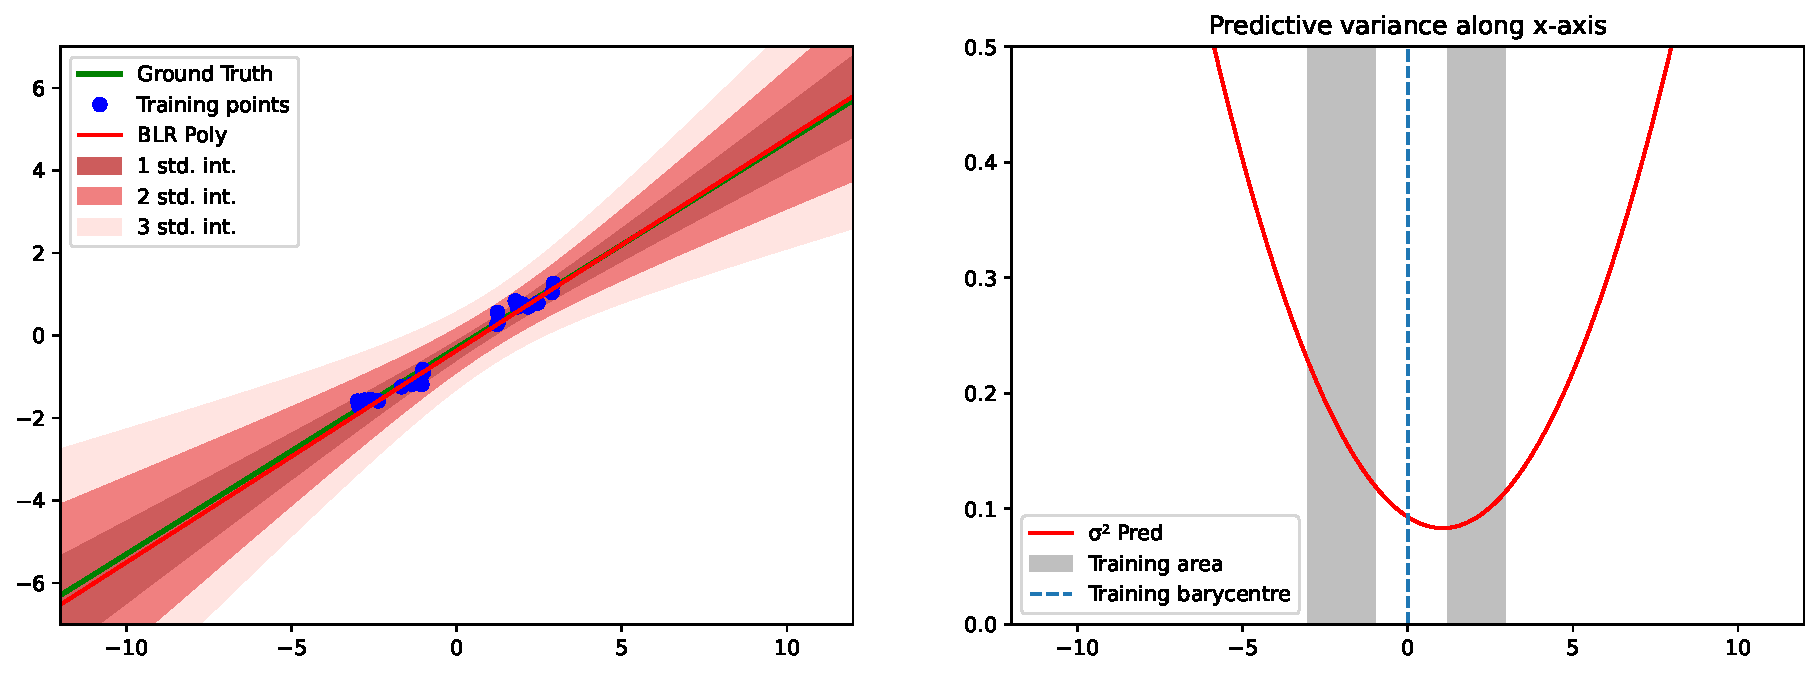
\includegraphics[width=0.95\textwidth]{phi_linear_hole.pdf}
    \caption{Visualization of predictive distribution of a linear dataset featuring a ''hole'' using Bayesian Linear Regression.}
    \label{fig:phi_linear_hole}
\end{figure}

\section{Non Linear models}

In this section, we apply the theoretical concepts learned in the previous section to more intricate datasets. The goal is to gain insights into the significance of the selected basis function and its impact on the behavior of predictive variance.

\subsection{Polynomial basis functions}

\paragraph*{2.2. Code and visualize results on sinusoidal dataset using polynomial basis functions. What can you say about the predictive variance?}

Figures \ref{fig:phi_polynomial} and \ref{fig:phi_polynomial_hole} illustrate a comparison between the predictions made by a Bayesian Polynomial Regression model and the actual ground truth. Given that the closed-form solution for the posterior and predictive distribution in $\Phi$ is similar to the linear case, we can draw the same conclusions: as we move further away from our training data, uncertainty increases. However, due to our polynomial kernel, the model exhibits higher predictive variance (i.e. higher epistemic uncertainity) when considering the values alone. Nevertheless, thanks to this basis function, our model demonstrates the ability to capture more intricate patterns, such as those resembling a sinusoidal function. It's worth noting that beyond the training data points, the model struggles to generalize, as it lacks the necessary data points to accurately capture the periodic nature of the sinusoidal ground truth. % je ne sais pas s'il y a plus de choses à dire pour la predictive variance, à part pourquoi elle "explose" moins vite à gauche qu'à droite..?

\begin{figure}[H]
    \centering
    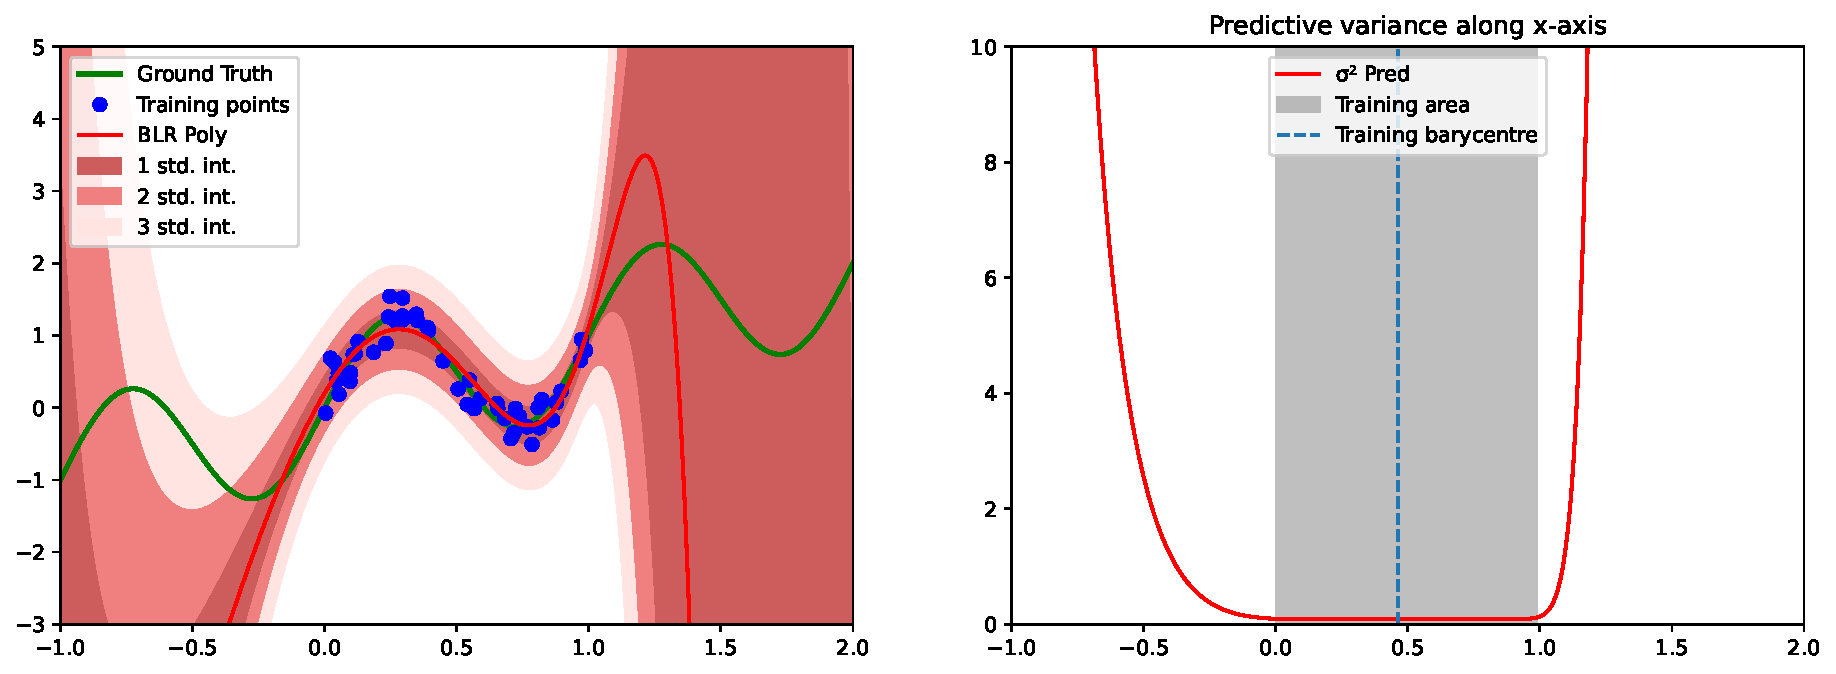
\includegraphics[width=0.95\textwidth]{phi_polynomial.pdf}
    \caption{Visualization of predictive distribution of a sinusoidal dataset using Bayesian Polynomial Regression.}
    \label{fig:phi_polynomial}
\end{figure}

Furthermore, we decided to explore the effects of providing data points that are more dispersed and less abundant, as shown in \Cref{fig:phi_polynomial_hole}. Unsurprisingly, we observe that the variance around these small clusters is minimal, and as we move away from these regions, the variance increases. This phenomenon highlights the strength of these models: when given data, they become increasingly confident in specific areas. Therefore, in the context of uncertainty, we can gradually narrow down our desired outcomes by continuously adding more data points over time.

\begin{figure}[H]
    \centering
    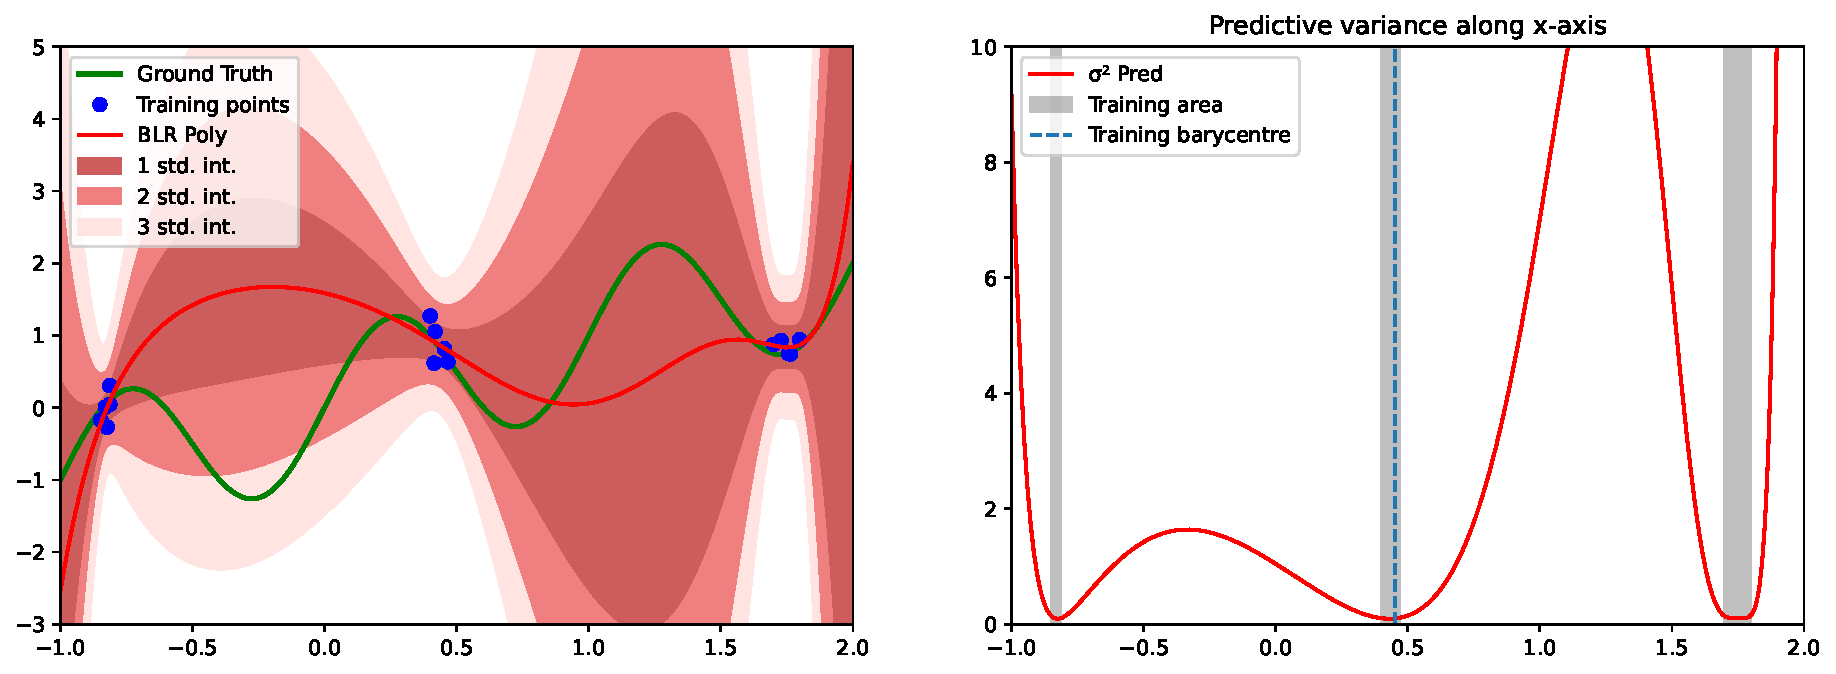
\includegraphics[width=0.95\textwidth]{phi_polynomial_hole.pdf}
    \caption{Visualization of predictive distribution of a sinusoidal dataset featuring ''holes'' and sparse data points using Bayesian Polynomial Regression.}
    \label{fig:phi_polynomial_hole}
\end{figure}

\subsection{Gaussian basis functions}

\paragraph*{2.4. Code and visualize results on sinusoidal dataset using Gaussian basis functions. What can you say this time about the predictive variance?}

Figures \ref{fig:phi_gaussian} and \ref{fig:phi_gaussian_hole} offer a comparison between the predictions generated by an RBF Gaussian Regression model and the actual ground truth. In contrast to the previous two models, our analysis leads to distinct conclusions. Notably, the predictive variance is at its highest not in regions far from the training barycenter. This is because the mean encompasses the entire range of data, resulting in predictive variance being concentrated solely within this zone. Beyond this range, predictive variance diminishes, which we explain in the next question. The predictive variance demonstrates a fluctuating pattern, marked by peaks and troughs corresponding to regions where the density of training points varies. Consequently, the model closely adheres to the mean of the training data, which is evident in its impact on the behavior of the sinusoidal curves.

% ptit shift dans la moyenne a un endroit et ça modifie la tête de la sinusoide qui dévie avant de reprendre une tête de sinusoide, donc très fitted sur les données, moyenne des données

\begin{figure}[H]
    \centering
    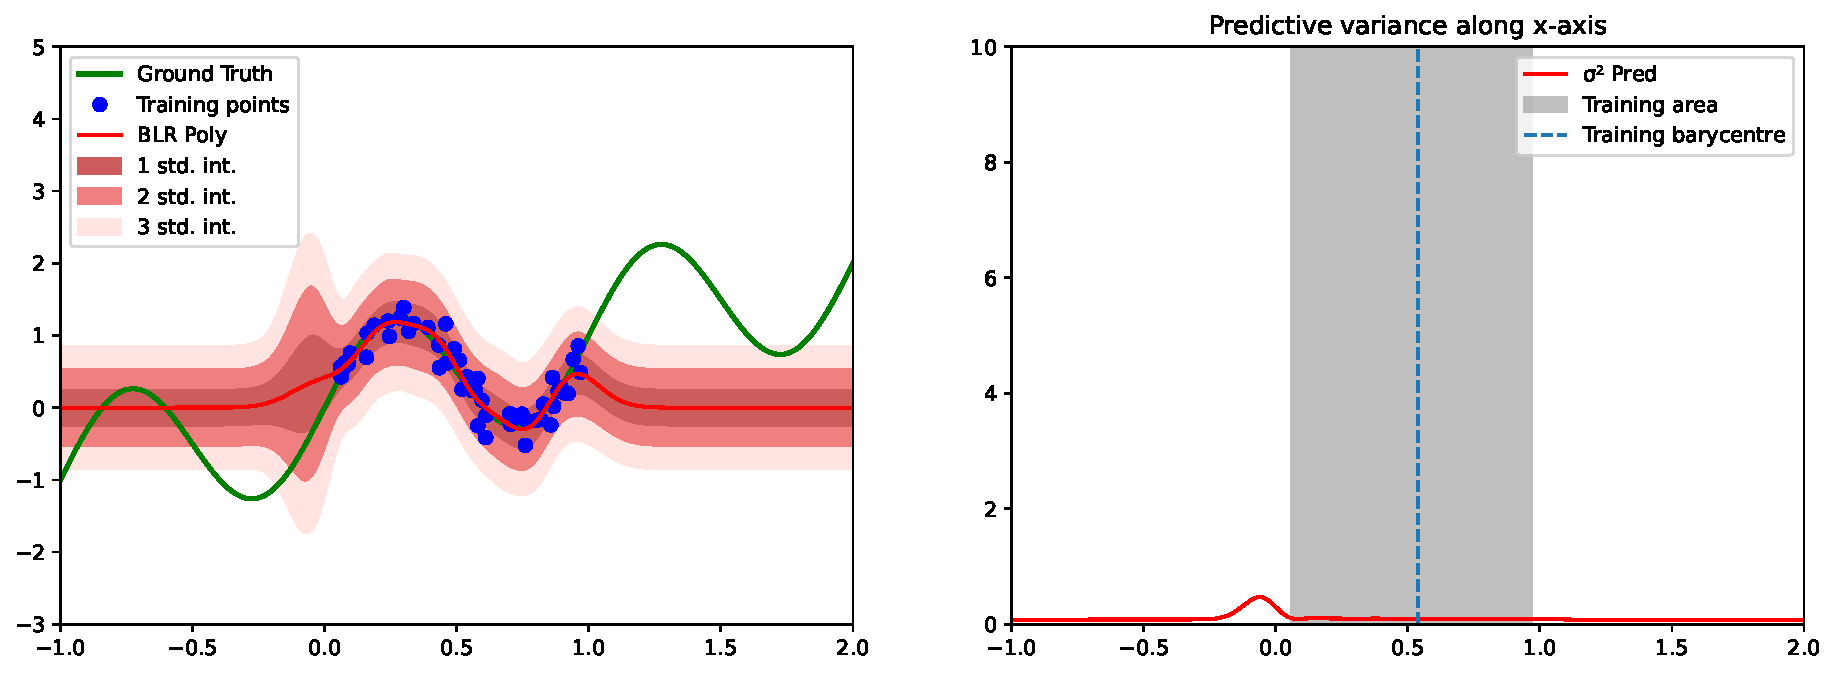
\includegraphics[width=0.95\textwidth]{phi_gaussian.pdf}
    \caption{Visualization of predictive distribution of a sinusoidal dataset using RBF Gaussian Regression, where we set $\mu \in [0.0, 1.0]$ and $M = 9$.}
    \label{fig:phi_gaussian}
\end{figure}

When we visualize our model with a reduced number of data points, it reinforces what has been discussed and emphasizes the role of hyperparameters. Notably, the model struggles to capture the information provided by the data points at the extremes, as they lie outside the range of the specified mean. Nonetheless, the predictive variance exhibits a significant increase as anticipated in regions where no data points are present.

\begin{figure}[H]
    \centering
    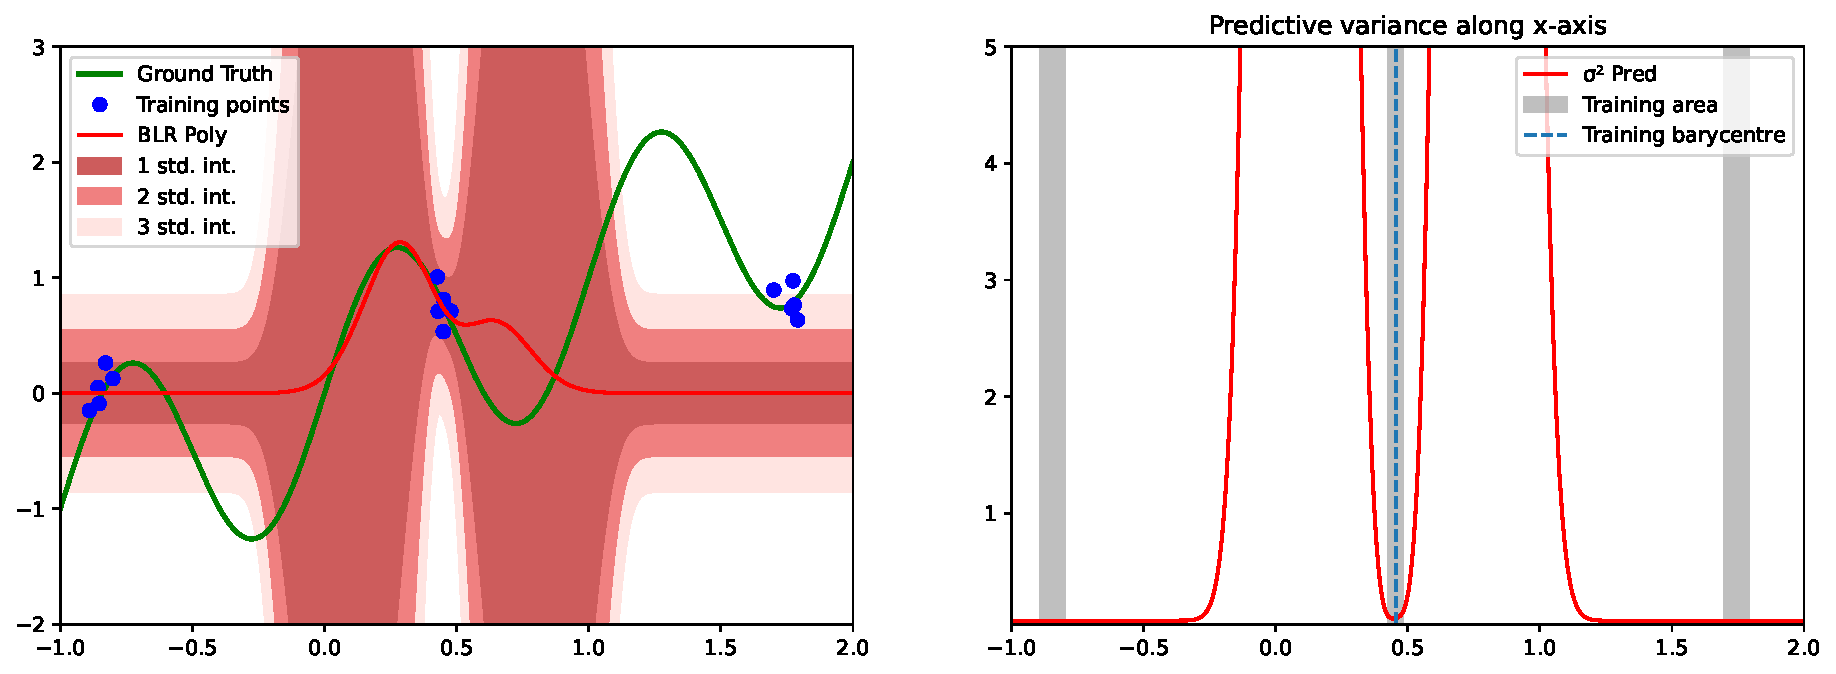
\includegraphics[width=0.95\textwidth]{phi_gaussian_hole.pdf}
    \caption{Visualization of predictive distribution of a sinusoidal dataset featuring ''holes'' and sparse data points using RBF Gaussian Regression, where we set $\mu \in [0.0, 1.0]$ and $M = 9$.}
    \label{fig:phi_gaussian_hole}
\end{figure}

\paragraph*{2.5. Explain why in regions far from training distribution, the predictive variance converges to this value when using localized basis functions such as Gaussians.}

Let us recall the definition of the Radial Basis Function:
\[ \Phi_j(x_i) = \exp\left( - \frac{(x_i - \mu_j)^2}{2s^2} \right), \]
where $\mu_j$ represents the center of the j-th Gaussian basis function and $s$ is a parameter controlling the spread of the Gaussian.

The primary observation is that this Gaussian function reaches its maximum at its center, where $x = \mu_j$ since $(x - \mu_j)^2 = 0$. As the distance $(x - \mu_j)^2$ increases, the exponential term rapidly tends toward zero. So, if $x^*$ is far from $\mu_j$, we can approximate $\Phi_j(x^*) \approx 0$. As a result, when we multiply this vector by the covariance matrix and its transpose, the epistemic uncertainty converges toward zero. Therefore, $\sigma_{\text{pred}}^2 = \beta^{-1} + \Phi(x^*)^T \Sigma \Phi(x^*) \approx \beta^{-1}$, signifying that the predictive variance is effectively reduced to aleatoric uncertainty. This can be observed in Figures \ref{fig:phi_gaussian} and \ref{fig:phi_gaussian_hole}, where $\sigma_{\text{pred}}^2 = \beta^{-1} = 0.08$.

Consequently, $\mu$ and $M$ are two critical hyperparameters (with $s$ derived from them), and their selection should be based on our data. For instance, setting $\mu \in [-2, 2]$ without changing $M$ yields significantly improved results, as demonstrated in Figures \ref{fig:phi_gaussian_modified_distance} and \ref{fig:phi_gaussian_hole_modified_distance}. We observe that these outcomes outperform the polynomial approach while maintaining similarity, thereby highlighting the robustness and popularity of the RBF kernel.

\begin{figure}[H]
    \centering
    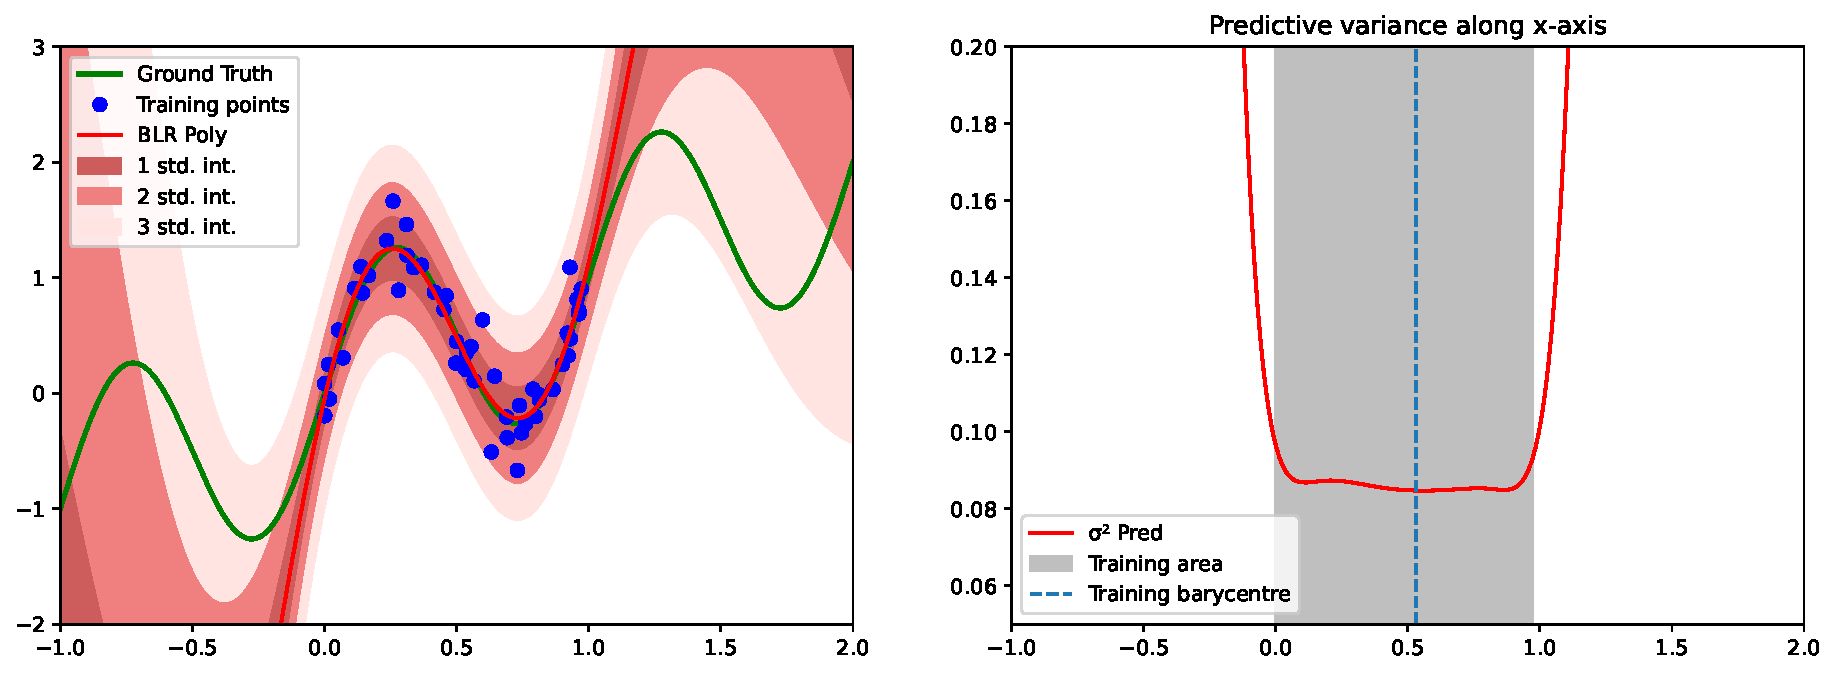
\includegraphics[width=0.95\textwidth]{phi_gaussian_modified_distance.pdf}
    \caption{Visualization of predictive distribution of a sinusoidal dataset using RBF Gaussian Regression, where we set $\mu \in [-2.0, 2.0]$ and $M = 9$.}
    \label{fig:phi_gaussian_modified_distance}
\end{figure}

\begin{figure}[H]
    \centering
    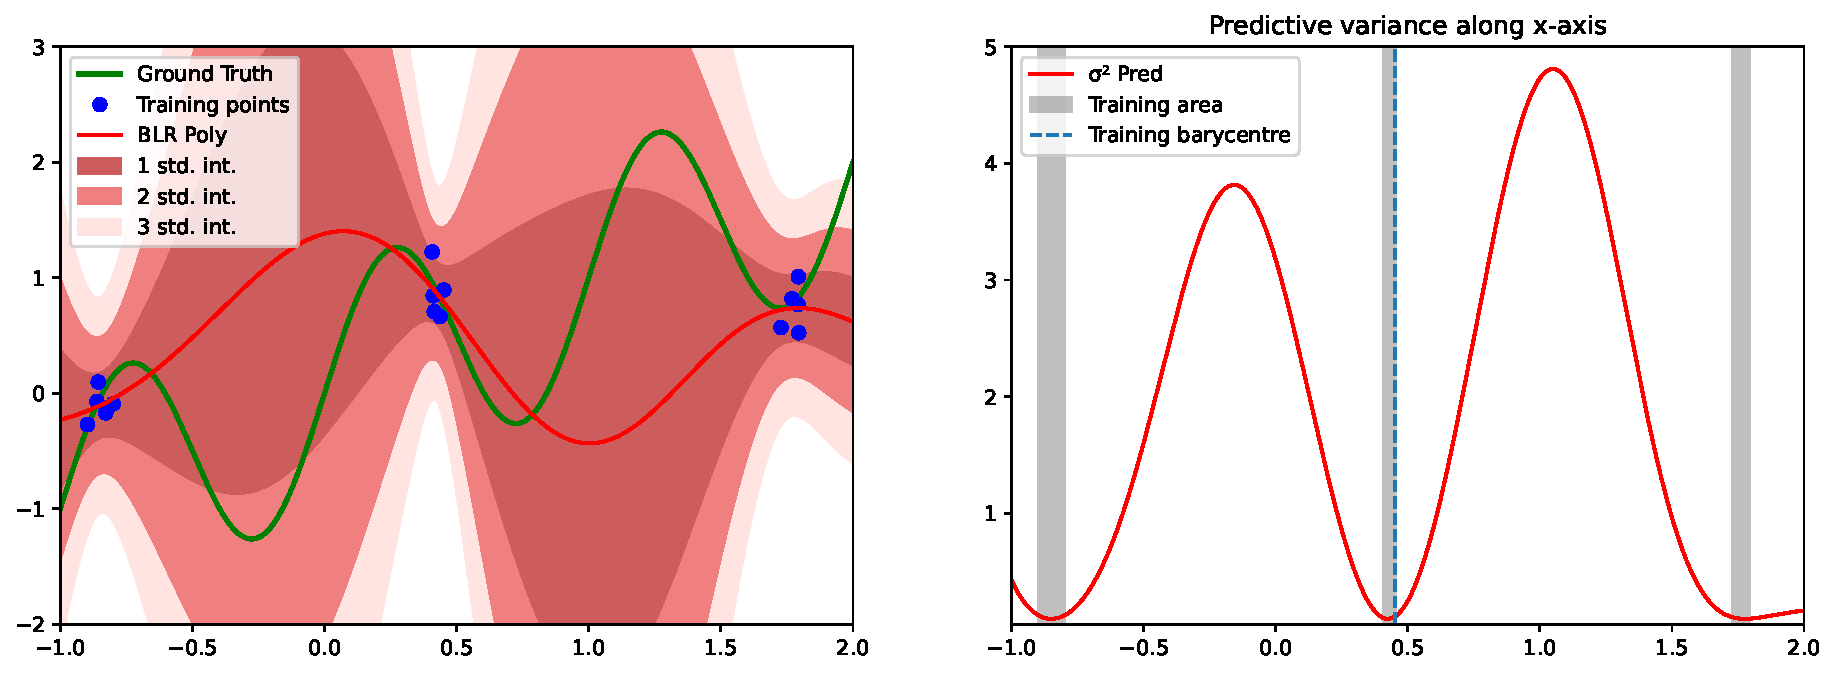
\includegraphics[width=0.95\textwidth]{phi_gaussian_hole_modified_distance.pdf}
    \caption{Visualization of predictive distribution of a sinusoidal dataset using RBF Gaussian Regression, where we set $\mu \in [-2.0, 2.0]$ and $M = 9$.}
    \label{fig:phi_gaussian_hole_modified_distance}
\end{figure}